% Options for packages loaded elsewhere
\PassOptionsToPackage{unicode}{hyperref}
\PassOptionsToPackage{hyphens}{url}
\PassOptionsToPackage{dvipsnames,svgnames,x11names}{xcolor}
%
\documentclass[
  letterpaper,
  DIV=11,
  numbers=noendperiod]{scrreprt}

\usepackage{amsmath,amssymb}
\usepackage{iftex}
\ifPDFTeX
  \usepackage[T1]{fontenc}
  \usepackage[utf8]{inputenc}
  \usepackage{textcomp} % provide euro and other symbols
\else % if luatex or xetex
  \usepackage{unicode-math}
  \defaultfontfeatures{Scale=MatchLowercase}
  \defaultfontfeatures[\rmfamily]{Ligatures=TeX,Scale=1}
\fi
\usepackage{lmodern}
\ifPDFTeX\else  
    % xetex/luatex font selection
\fi
% Use upquote if available, for straight quotes in verbatim environments
\IfFileExists{upquote.sty}{\usepackage{upquote}}{}
\IfFileExists{microtype.sty}{% use microtype if available
  \usepackage[]{microtype}
  \UseMicrotypeSet[protrusion]{basicmath} % disable protrusion for tt fonts
}{}
\makeatletter
\@ifundefined{KOMAClassName}{% if non-KOMA class
  \IfFileExists{parskip.sty}{%
    \usepackage{parskip}
  }{% else
    \setlength{\parindent}{0pt}
    \setlength{\parskip}{6pt plus 2pt minus 1pt}}
}{% if KOMA class
  \KOMAoptions{parskip=half}}
\makeatother
\usepackage{xcolor}
\setlength{\emergencystretch}{3em} % prevent overfull lines
\setcounter{secnumdepth}{5}
% Make \paragraph and \subparagraph free-standing
\ifx\paragraph\undefined\else
  \let\oldparagraph\paragraph
  \renewcommand{\paragraph}[1]{\oldparagraph{#1}\mbox{}}
\fi
\ifx\subparagraph\undefined\else
  \let\oldsubparagraph\subparagraph
  \renewcommand{\subparagraph}[1]{\oldsubparagraph{#1}\mbox{}}
\fi


\providecommand{\tightlist}{%
  \setlength{\itemsep}{0pt}\setlength{\parskip}{0pt}}\usepackage{longtable,booktabs,array}
\usepackage{calc} % for calculating minipage widths
% Correct order of tables after \paragraph or \subparagraph
\usepackage{etoolbox}
\makeatletter
\patchcmd\longtable{\par}{\if@noskipsec\mbox{}\fi\par}{}{}
\makeatother
% Allow footnotes in longtable head/foot
\IfFileExists{footnotehyper.sty}{\usepackage{footnotehyper}}{\usepackage{footnote}}
\makesavenoteenv{longtable}
\usepackage{graphicx}
\makeatletter
\def\maxwidth{\ifdim\Gin@nat@width>\linewidth\linewidth\else\Gin@nat@width\fi}
\def\maxheight{\ifdim\Gin@nat@height>\textheight\textheight\else\Gin@nat@height\fi}
\makeatother
% Scale images if necessary, so that they will not overflow the page
% margins by default, and it is still possible to overwrite the defaults
% using explicit options in \includegraphics[width, height, ...]{}
\setkeys{Gin}{width=\maxwidth,height=\maxheight,keepaspectratio}
% Set default figure placement to htbp
\makeatletter
\def\fps@figure{htbp}
\makeatother
% definitions for citeproc citations
\NewDocumentCommand\citeproctext{}{}
\NewDocumentCommand\citeproc{mm}{%
  \begingroup\def\citeproctext{#2}\cite{#1}\endgroup}
\makeatletter
 % allow citations to break across lines
 \let\@cite@ofmt\@firstofone
 % avoid brackets around text for \cite:
 \def\@biblabel#1{}
 \def\@cite#1#2{{#1\if@tempswa , #2\fi}}
\makeatother
\newlength{\cslhangindent}
\setlength{\cslhangindent}{1.5em}
\newlength{\csllabelwidth}
\setlength{\csllabelwidth}{3em}
\newenvironment{CSLReferences}[2] % #1 hanging-indent, #2 entry-spacing
 {\begin{list}{}{%
  \setlength{\itemindent}{0pt}
  \setlength{\leftmargin}{0pt}
  \setlength{\parsep}{0pt}
  % turn on hanging indent if param 1 is 1
  \ifodd #1
   \setlength{\leftmargin}{\cslhangindent}
   \setlength{\itemindent}{-1\cslhangindent}
  \fi
  % set entry spacing
  \setlength{\itemsep}{#2\baselineskip}}}
 {\end{list}}
\usepackage{calc}
\newcommand{\CSLBlock}[1]{\hfill\break\parbox[t]{\linewidth}{\strut\ignorespaces#1\strut}}
\newcommand{\CSLLeftMargin}[1]{\parbox[t]{\csllabelwidth}{\strut#1\strut}}
\newcommand{\CSLRightInline}[1]{\parbox[t]{\linewidth - \csllabelwidth}{\strut#1\strut}}
\newcommand{\CSLIndent}[1]{\hspace{\cslhangindent}#1}

\KOMAoption{captions}{tableheading}
\makeatletter
\@ifpackageloaded{bookmark}{}{\usepackage{bookmark}}
\makeatother
\makeatletter
\@ifpackageloaded{caption}{}{\usepackage{caption}}
\AtBeginDocument{%
\ifdefined\contentsname
  \renewcommand*\contentsname{Table of contents}
\else
  \newcommand\contentsname{Table of contents}
\fi
\ifdefined\listfigurename
  \renewcommand*\listfigurename{List of Figures}
\else
  \newcommand\listfigurename{List of Figures}
\fi
\ifdefined\listtablename
  \renewcommand*\listtablename{List of Tables}
\else
  \newcommand\listtablename{List of Tables}
\fi
\ifdefined\figurename
  \renewcommand*\figurename{Figure}
\else
  \newcommand\figurename{Figure}
\fi
\ifdefined\tablename
  \renewcommand*\tablename{Table}
\else
  \newcommand\tablename{Table}
\fi
}
\@ifpackageloaded{float}{}{\usepackage{float}}
\floatstyle{ruled}
\@ifundefined{c@chapter}{\newfloat{codelisting}{h}{lop}}{\newfloat{codelisting}{h}{lop}[chapter]}
\floatname{codelisting}{Listing}
\newcommand*\listoflistings{\listof{codelisting}{List of Listings}}
\makeatother
\makeatletter
\makeatother
\makeatletter
\@ifpackageloaded{caption}{}{\usepackage{caption}}
\@ifpackageloaded{subcaption}{}{\usepackage{subcaption}}
\makeatother
\ifLuaTeX
  \usepackage{selnolig}  % disable illegal ligatures
\fi
\usepackage{bookmark}

\IfFileExists{xurl.sty}{\usepackage{xurl}}{} % add URL line breaks if available
\urlstyle{same} % disable monospaced font for URLs
\hypersetup{
  pdftitle={Electromagnetism},
  pdfauthor={Claire Greenland},
  colorlinks=true,
  linkcolor={blue},
  filecolor={Maroon},
  citecolor={Blue},
  urlcolor={Blue},
  pdfcreator={LaTeX via pandoc}}

\title{Electromagnetism}
\author{Claire Greenland}
\date{2024-03-25}

\begin{document}
\maketitle

\renewcommand*\contentsname{Table of contents}
{
\hypersetup{linkcolor=}
\setcounter{tocdepth}{2}
\tableofcontents
}
\bookmarksetup{startatroot}

\chapter*{Preface}\label{preface}
\addcontentsline{toc}{chapter}{Preface}

\markboth{Preface}{Preface}

This is a Quarto book.

To learn more about Quarto books visit
\url{https://quarto.org/docs/books}.

Put a nice introduction here introducing the subject of electromagnetism
:D

\bookmarksetup{startatroot}

\chapter{Electrostatics - Charges, Forces \&
Fields}\label{electrostatics---charges-forces-fields}

\newcommand{\l}{\mathrm{\mathbf{l}}}
\newcommand{\E}{\mathrm{\mathbf{E}}}
\newcommand{\F}{\mathrm{\mathbf{F}}}
\newcommand{\r}{\mathrm{\mathbf{r}}}
\newcommand{\B}{\mathrm{\mathbf{B}}}
\newcommand{\A}{\mathrm{\mathbf{A}}}
\newcommand{\x}{\mathrm{\mathbf{x}}}
\newcommand{\y}{\mathrm{\mathbf{y}}}
\newcommand{\z}{\mathrm{\mathbf{z}}}
\newcommand{\v}{\mathrm{\mathbf{v}}}
\newcommand{\p}{\mathrm{\mathbf{p}}}
\newcommand{\d}{\mathrm{\mathbf{d}}}

\newcommand{\a}{\mathrm{\mathbf{a}}}
\newcommand{\b}{\mathrm{\mathbf{b}}}
\newcommand{\I}{\mathrm{\mathbf{I}}}
\newcommand{\dd}{\mathrm{d}}

\emph{Recommended reading}: Griffiths Section 2.1 (and 2.2 if you want
some bonus reading about stuff that will be important later)

\section{Pre-lecture problem}\label{pre-lecture-problem}

Griffiths Problem 1.7

\section{Electric Charges}\label{electric-charges}

Electric charge is a fundamental property of matter. Many fundamental
particles (such as electrons and protons) have charge. However,
macroscopic objects can also be charged due to having a distribution of
charged particles on them that has a small imbalance in charge - we
might describe these as ``charged objects''.

Charge gives rise to electric fields, and hence to the electric forces
experienced between charged particles or objects.

Charge can be either a positive or negative quantity. ``Like'' charges
(charges with the same sign) repel each other, and opposite charges
attract.

Charge is quantized and comes in integer multiples of the elementary
charge \(e\) which has an approximate value of
\(1.602 \times 10 ^{-19}\) Coulombs. Electrons carry a charge of \(-e\),
and protons carry a charge of \(+e\). Charges measured in laboratories
are always multiples of \(e\) but the quarks inside protons and neutrons
and other hadrons have charges that are fractions of this elementary
charge.

Charge is conserved - or more specifically, the total charge in an
isolated system is conserved. (At least, this has been the case in all
the particle interactions physicists have so far observed.) Hence,
charge can be neither created nor destroyed, but can only be transferred
from one object to another.

\textbf{Gravitational charge:} there is one type of gravitational
charge, which is mass/energy. Gravitational charges attract. We don't
know about quantization of mass. (You can probably spend many hours on
the internet reading different opinions on this). Mass/Energy is
conserved and all everyday objects are gravitationally charged so they
all attract each other, but gravity is very weak--we can easily pick up
bits of paper with an electrically charged rod when rather few electrons
have been moved.

\section{Some definitions and important
notation}\label{some-definitions-and-important-notation}

Here I will briefly explain some notation and definitions I will use in
this course for setting up and solving problems involving electric
charges.

Consider the following ensemble of charges:

\begin{figure}[H]

{\centering 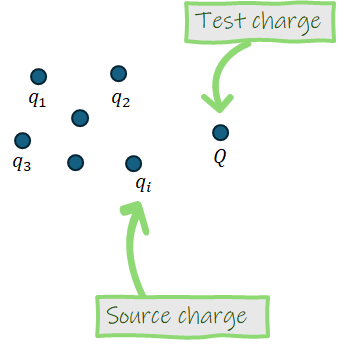
\includegraphics{Figures/sourcetest_definitions.png}

}

\caption{Some charges.}

\end{figure}%

We define the charges \(q_1\), \(q_2\), \(q_3\)\ldots{} \(q_i\) as
source charges, meaning that these are the charges that produce the
electric field for the purpose of the problem. We define \(Q\) as the
test charge, which means it is the charge that is experiencing the
effects of the electric field produced by the source charge(s). It is
important to note that any charge can be a source or a test charge,
there is no fundamental difference between them. ``Source'' and ``test''
are simply names that we give charges when setting up a problem, so that
we can more easily define and solve the problem.

Throughout this course you will also see the terms ``source point'' and
``field point''. The source point is the location of the source
charge(s), while the field point is essentially the location of the test
charge - so when we are solving problems, this is the point at which we
are measuring the field, potential, etc. The source point is given by
the vector \(\mathrm{\mathbf{r}}'\) and the field point is given by the
vector \(\mathrm{\mathbf{r}}\), while the separation between the two
point is given by the vector \(r_s\). (Please note that the Griffiths
uses slightly different notation - for the separation vector it uses a
curly script ``r'', I did not use this as there is no way of making that
symbol in Latex.) If there is no test charge in the problem (for example
if we are computing the electric field of a source charge), the field
point is the point at which we are measuring the field - it is the point
where a test charge would be if there was one.

\begin{figure}[H]

{\centering 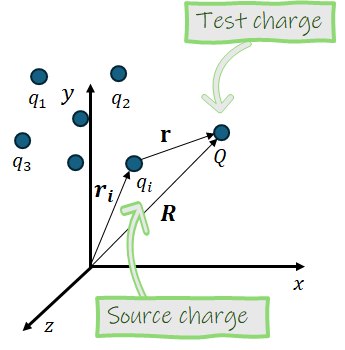
\includegraphics{Figures/axes_r_definitions.png}

}

\caption{Some charges, overlaid with axes showing the definition of
\(\mathrm{\mathbf{r}}\), the vector separation between the source and
test charges.}

\end{figure}%

\section{Electric Forces \& Coulomb's
Law}\label{electric-forces-coulombs-law}

All charges produce electric fields, and other charges that are in the
prescence of this field experience a force as a result.

The force on a test charge \(Q\), exerted by a source charge \(q\), is
given by Coulomb's Law, which is as follows:
\[ F = \frac{1}{4\pi \epsilon_0} \frac{q Q}{r_s^2} \hat{\mathrm{\mathbf{r}}_s} \]

where:

\begin{itemize}
\tightlist
\item
  \(\hat{\mathrm{\mathbf{r}}}\) is the unit vector in the direction of
  the force, which points from \(q\) to \(Q\).
\item
  \(r\) is the separation between \(q\) and \(Q\).
\item
  \(\epsilon_0\) is a physical constant known as the
  \bf{permittivity of free space}.  $\epsilon_0 \approx 8.85 \times 10^{-12}$ Fm $^{-1}$ (farads per metre). 
\end{itemize}

If \(q\) and \(Q\) have the same sign (like charges) the force is
repulsive (\(\mathrm{\mathbf{F}}\) is a positive quantity); if \(q\) and
\(Q\) have different signs, the force is attractive
(\(\mathrm{\mathbf{F}}\) is a negative quantity).

\section{Electric Field}\label{electric-field}

The electric field \(\mathrm{\mathbf{E}}\) produced by a charge (or
charged object/charge distribution) is a vector field that represents
the force per unit charge experienced by a positive test charge placed
at a particular point in space:

\[ \mathrm{\mathbf{E}}= \frac{\mathrm{\mathbf{F}}}{Q} \]

\noindent which can be rearranged to the more familiar form
\(\mathrm{\mathbf{F}}= Q \mathrm{\mathbf{E}}\).

\(\mathbf{E}\) has units of Vm\(^{-1}\) or NC\(^{-1}\).

The electric field is normally represented by field lines that indicate
the direction of the field. The direction of the field is determined by
what a positive test charge will do. That's why field lines point
towards negative charges - that's the direction a positive charge would
travel if it encountered the field of a negative charge. The density of
lines/arrows indicates the strength of the field at a point. You may
also see fields drawn where the size of the arrows represents the
electric field strength. The diagram below shows the electric field
lines for two positive point charges of the same magnitude.

\begin{figure}[H]

{\centering 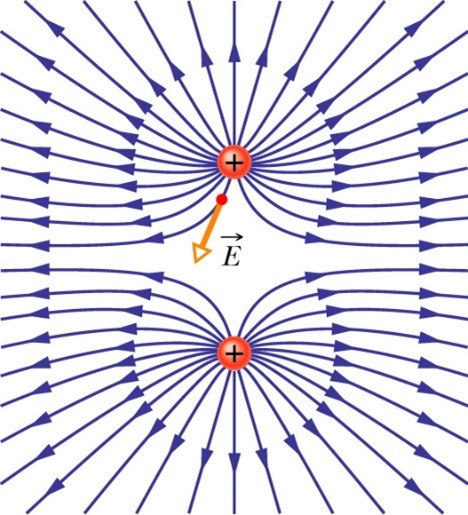
\includegraphics{Figures/Efield_like.png}

}

\caption{Representation of the electric field surrounding two positive
charges.}

\end{figure}%

Most important rules for field lines:

\begin{itemize}
\item
  Lines begin on positive charges and end on negative charges.
\item
  Lines never intersect.
\item
  Lines are symmetric as they leave the charges.
\end{itemize}

\section{Superposition Principle}\label{superposition-principle}

The principle of superposition states that ``the interaction between any
two charges is completely unaffected by the presence of others''. This
means that the total force on a test charge can be computed by
calculating the force on the test charge due to each source charge
separately, then adding up the contributions, as follows:

\[ \mathrm{\mathbf{F}}_{tot} = \sum_i \mathrm{\mathbf{F}}_i \]

The same applies to the electric field, which can be calculated for any
given point in space as a sum of the electric field at that point from
all the source charges:
\[ \mathrm{\mathbf{E}}_{tot} = \sum_i \mathrm{\mathbf{E}}_i \]

\section{Continuous charge
distributions}\label{continuous-charge-distributions}

\section{Summary}\label{summary}

Electric charges create electric fields, which exert forces on other
charges. Coulomb's Law describes the force between point charges.

\section{Bonus content: vector
fields}\label{bonus-content-vector-fields}

\subsection{What is a field?}\label{what-is-a-field}

\emph{Recommended reading:}

A field is a region of space, where property of that space is
characterized by either a number (a scalar field) or by three numbers (a
vector field).

The concept of a field circumvents the problem of action at a distance,
where one inanimate object is ``aware'' that another has arrived. We
understand that the first body sets up a field and the second body
interacts with the first via this field.

\subsection{Scalar and vector fields}\label{scalar-and-vector-fields}

A scalar field is characterized at each point by a single number.
e.g.~the temperature, \(T\), at each position in a block of metal heated
at some places and cooled at others.

\begin{figure}[H]

{\centering 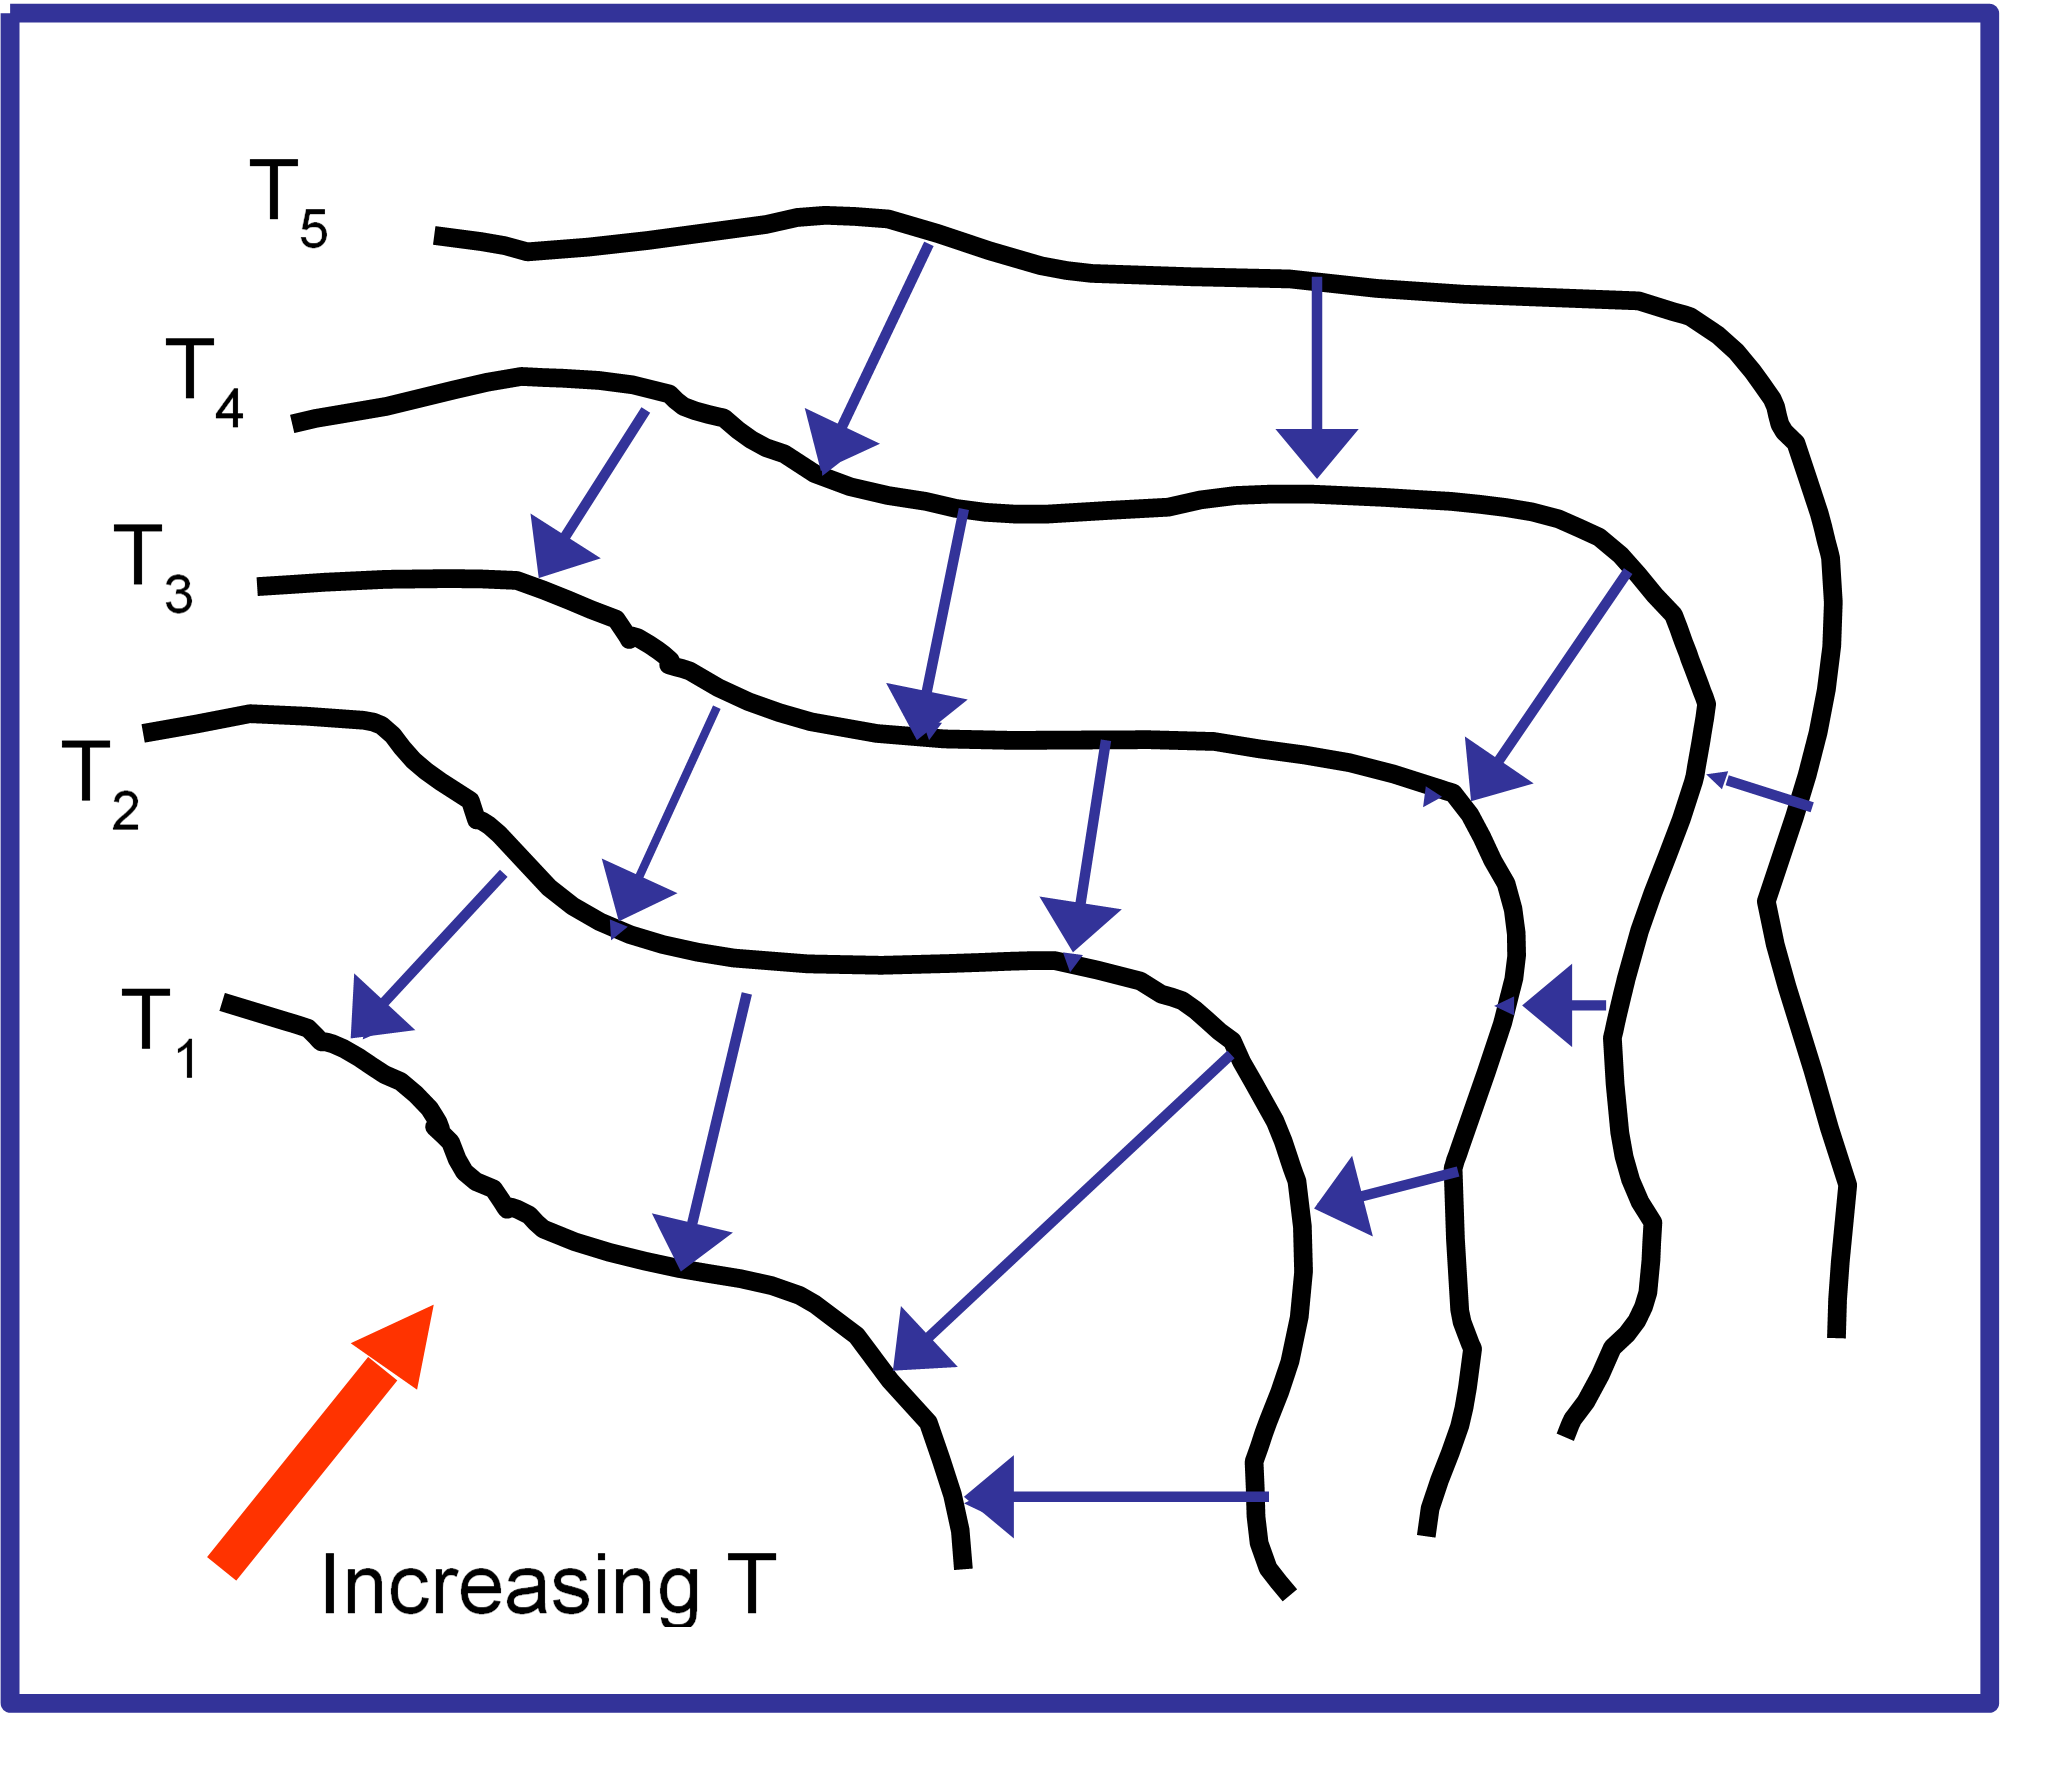
\includegraphics[width=80mm,height=\textheight]{Figures/isotherms.png}

}

\caption{A representation of a temperature field. Isotherms at different
temperatures are black lines; blue arrows show the direction of heat
flow, which is always perpendicular to the isotherms.}

\end{figure}%

\(T\) is a function of position i.e.~\(T = T(x,y,z)\). At every point we
can measure the scalar value of the temperature \(T\). The black lines
represent isotherms i.e.~lines where the temperature is constant
(\(T_1 < T_2 < T_3 < T_4 < T_5\)). Heat flow (blue arrows) is
perpendicular to the contours of constant temperature - the isotherms
(\(T_1\), \(T_2\) etc). The magnitude of the heat flow is proportional
to the temperature gradient, so that the heat flow is larger when
isotherms are closer together.

The scalar temperature field has an associated vector field, because at
any point, the heat flow is a vector, the \textbf{magnitude} and
\textbf{direction} of which depend on position. Heat flow is therefore a
vector field which is related to the scalar field of temperature. The
vector gradient of the field of heat flow depends on the temperature at
each point.

\subsection{Link between scalar and vector
field}\label{link-between-scalar-and-vector-field}

\emph{Recommended reading:}

For the scalar temperature field \(T(x,y,z)\) the vector describing the
direction and the magnitude of the maximum temperature gradient is:

\begin{equation}
 \text{Grad} \; T = \nabla T = \frac{\partial T} {\partial x} \hat{\mathbf{i}} + \frac{\partial T}{\partial y} \hat{\mathbf{j}} + \frac{\partial T}{\partial y} \hat{\mathbf{k}}
\end{equation}

The heat flow is a vector given by \(\mathbf{Q} = -k \nabla T\); the
minus sign is because heat flows from high temperature to low
temperature.

In general, for a scalar potential
\(-\nabla \phi = \frac{\partial \phi} {\partial x} \hat{\mathbf{i}} + \frac{\partial \phi}{\partial y} \hat{\mathbf{j}} + \frac{\partial \phi}{\partial y} \hat{\mathbf{k}}\)
describes the magnitude and direction of the physical effects of the
potential, with an appropriate constant if needed. In the case of the
electric field if the electric potential is \(V\) then the vector field
\(\mathbf{E} = -\nabla V\).

As an example, the gravitational field can be obtained from the
gravitational potential. The scalar gravitational potential energy is
given by \(U = mgz\) near the Earth's surface, where \(z\) is the
height. The gravitational potential is \(U/m = gz\). The gravitational
field is \(-\nabla(gz)=-g \hat{\mathbf{k}}\).

\subsection{Other operations on
vectors}\label{other-operations-on-vectors}

The vector operator \(\nabla\) behaves as a vector. We have looked at
grad \(\nabla\phi\) where \(\phi\) is a scalar field. In Maxwell's
equations, which you cover next year, you will also meet \(\nabla\)
operating on the electric field \(\mathbf{E}\):

\(\nabla \cdot \mathbf{E}\) (div or divergence)

\(\nabla \times \mathbf{E}\) (curl or rotation)

Maxwell's equations are one of the great achievements of 19th century
Physics. They link the phenomena of electricity and magnetism and can be
used to derive an expression for the speed of light. Einstein said that
the theory of Relativity was rooted in Maxwell's equations. The
equations in their differential form are shown below and we will meet
these in more detail later in the course, along with the integral
versions of these laws.

\begin{equation}

\nabla \cdot \mathbf{E} = \frac{\rho}{\epsilon_0}
\end{equation}

\begin{equation}
\nabla \times \mathbf{E} = - \frac{\partial \mathbf{B}}{\partial t} 
\end{equation}

\begin{equation}
\nabla \cdot \mathbf{B} = 0
\end{equation}

\begin{equation}
\nabla \times \mathbf{B} = \frac{\mathbf{j}}{c^2 \epsilon_0} + \frac{1}{c^2} \frac{\partial \mathbf{E}}{\partial t}
\end{equation}

Source:
\url{http://www.clerkmaxwellfoundation.org/html/about_maxwell.html};\url{https://maxwells-equations.com/}

\section{Practice problems}\label{practice-problems}

\begin{enumerate}
\def\labelenumi{\arabic{enumi})}
\tightlist
\item
  (\emph{Griffiths Problem 2.2})
\end{enumerate}

In the lecture, we found the electric field (magnitude and direction) a
distance \(z\) above the midpoint between two equal charges, \(q\), a
distance \(d\) apart. We found that for distances \(z >> a\), as we
might expect the field appears like that of a single charge \(2q\).

Repeat the calculation of the electric field, but replace the charge on
the right with a negative charge (so we now have a dipole). Is there
anything interesting about this result? {[}Hint: try computing the field
for different ranges of \(z\)-values.{]}

\begin{enumerate}
\def\labelenumi{\arabic{enumi})}
\setcounter{enumi}{1}
\item
  Charges \(+Q\), \(+Q\) and \(-Q\) are arranged at the vertices of an
  equilateral triangle. What is the electric field at the centre of the
  triangle?
\item
  A charge \(Q\) is uniformly distributed along the circumference of a
  thin ring of radius \(R\). Find the electric field a distance \(z\)
  above the centre of the ring.
\end{enumerate}

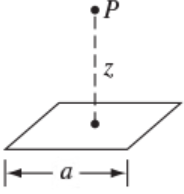
\includegraphics[width=1.04167in,height=\textheight]{Figures/L1_prob3.png}

:bulb: \textbf{Hint:} Have a look at Example 2.2 in the Griffiths.

\begin{enumerate}
\def\labelenumi{\arabic{enumi})}
\setcounter{enumi}{3}
\tightlist
\item
  (\emph{Griffiths Problem 2.6}) Find the electric field a distance
  \(z\) above the center of a flat circular disk of radius \(R\) (see
  figure below) that carries a uniform surface charge \(\sigma\). What
  does your formula give in the limit \(R \rightarrow \infty\)? Also
  check the case \(z >> R\).
\end{enumerate}

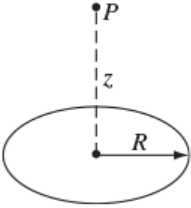
\includegraphics[width=1.04167in,height=\textheight]{Figures/L1_prob4.png}

\begin{enumerate}
\def\labelenumi{\arabic{enumi})}
\setcounter{enumi}{4}
\tightlist
\item
  Find the electric field at a distance \(z\) above the midpoint of a
  uniform line charge, of length \(2L\) and charge density \(\lambda\)
  (see figure below).
\end{enumerate}

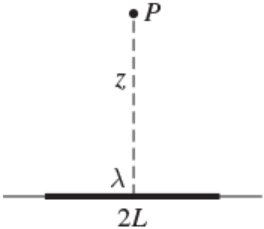
\includegraphics[width=2.08333in,height=\textheight]{Figures/L2_prob3.pdf}

\bookmarksetup{startatroot}

\chapter{Electric Potential}\label{electric-potential}

\newcommand{\l}{\mathrm{\mathbf{l}}}
\newcommand{\E}{\mathrm{\mathbf{E}}}
\newcommand{\F}{\mathrm{\mathbf{F}}}
\newcommand{\r}{\mathrm{\mathbf{r}}}
\newcommand{\B}{\mathrm{\mathbf{B}}}
\newcommand{\A}{\mathrm{\mathbf{A}}}
\newcommand{\x}{\mathrm{\mathbf{x}}}
\newcommand{\y}{\mathrm{\mathbf{y}}}
\newcommand{\z}{\mathrm{\mathbf{z}}}
\newcommand{\v}{\mathrm{\mathbf{v}}}
\newcommand{\p}{\mathrm{\mathbf{p}}}
\newcommand{\d}{\mathrm{\mathbf{d}}}

\newcommand{\a}{\mathrm{\mathbf{a}}}
\newcommand{\b}{\mathrm{\mathbf{b}}}
\newcommand{\I}{\mathrm{\mathbf{I}}}
\newcommand{\dd}{\mathrm{d}}

\emph{Recommended reading}: Griffiths Section 2.3

\section{Pre-lecture problem}\label{pre-lecture-problem-1}

Before you attempt this problem, it is recommended that you read through
the lecture notes, as well as Sections 2.3 and 2.2.4 of the Griffiths.
This question also requires some vector calculus, to which you have only
just been introduced. Do not worry if you can't do this question just
yet - we will go through it in the lecture.

One of these is an impossible electrostatic field. Which one?

\begin{enumerate}
\def\labelenumi{(\alph{enumi})}
\item
  \(\mathrm{\mathbf{E}}= k[ xy \hat{\mathrm{\mathbf{x}}} + 2yz \hat{\mathrm{\mathbf{y}}} + 3xz \hat{\mathrm{\mathbf{z}}} ]\)
\item
  \(\mathrm{\mathbf{E}}= k[ y^2 \hat{\mathrm{\mathbf{x}}} + (2xy + z^2)\hat{\mathrm{\mathbf{y}}} + 2yz \hat{\mathrm{\mathbf{z}}} ]\)
\end{enumerate}

For the \emph{possible} one, find the potential. Use the origin as your
reference point. Check your answer by computing \(\nabla V\).

{[}:bulb: \textbf{Hint:} you must select a specific path to integrate
along. The answer is \textbf{path-independent}, meaning that you will
get the same answer no matter what path you choose--however, it is
simply not possible to integrate unless you have a particular path in
mind.{]}

\section{Introduction to electric
potential}\label{introduction-to-electric-potential}

Electric potential is a scalar quantity associated with the electric
field. It is defined as the work done by an external force to bring a
unit positive charge to a particular point in space (for example, the
location of a test charge \(Q\)) from an arbitrary reference point. For
the purposes of this lecture course, we will choose infinity
(\(\infty\)) as our reference point - but please note that Griffiths
does not use infinity but rather uses the symbol \(\mathcal{O}\) to
denote an arbitrary reference point.

We will see later how the concept of electric potential simplifies many
calculations in electrostatics, particularly when dealing with electric
fields and potential energy.

\section{Definition of Electric
Potential}\label{definition-of-electric-potential}

The electric potential \(V\) at some displacement
\(\mathrm{\mathbf{r}}\) is given by

\[ V(\mathrm{\mathbf{r}}) = −\int_{\infty}^r \mathrm{\mathbf{E}}\cdot \mathrm{d}\mathrm{\mathbf{l}}\]

where \(\mathrm{\mathbf{E}}\) is the electric field, and
\(\mathrm{d}\mathrm{\mathbf{l}}\) is an infinitesimal displacement
vector along the path of the charge. As we have stated, the potential is
the work done per unit charge, therefore we can see how the above can be
derived. The work done by a force to bring an object from infinity to
point \(\mathrm{\mathbf{r}}\) is given by \$ \int\_\infty\^{}r
\mathrm{\mathbf{F}} \cdot \mathrm{d}\mathrm{\mathbf{l}}\$, therefore the
work done per unit charge is
\(\int_\infty^r \frac{\mathrm{\mathbf{F}}}{Q} \cdot \mathrm{d}\mathrm{\mathbf{l}}= \int_\infty^r \mathrm{\mathbf{E}}\cdot \mathrm{d}\mathrm{\mathbf{l}}\).
However, you will notice that the expression shown above is
\(- \int_\infty^r \mathrm{\mathbf{E}}\cdot \mathrm{d}\mathrm{\mathbf{l}}\)
- by convention, we add a minus sign because the direction of the
electric field is the direction of \emph{decreasing} potential. Let me
explain this. We have seen in the previous lecture that electric field
lines point away from a positive charge. If we place a positive test
charge in the vicinity of another positive charge, the test charge will
move away, in the direction of the electric field. This is the direction
of decreasing potential because the charge loses potential energy as it
moves away. Hence, the electric field points in the direction of
decreasing potential, so the expression for potential must be the
negative of the electric field.

\section{Potential Difference}\label{potential-difference}

The potential difference \(V_{ab}\) between two points
\(\mathrm{\mathbf{a}}\) and \(\mathrm{\mathbf{b}}\) is given by:

\[
\begin{split} 
V_{ab} & = V(\mathrm{\mathbf{b}}) − V(\mathrm{\mathbf{a}}) \\
& = -\int_{\infty}^{\mathrm{\mathbf{b}}} \mathrm{\mathbf{E}}\cdot \mathrm{d} \mathrm{\mathbf{l}}+ \int_{\infty}^{\mathrm{\mathbf{a}}} \mathrm{\mathbf{E}}\cdot \mathrm{d} \mathrm{\mathbf{l}}\\
& = -\int_{\infty}^{\mathrm{\mathbf{b}}} \mathrm{\mathbf{E}}\cdot \mathrm{d} \mathrm{\mathbf{l}}- \int_{\mathrm{\mathbf{a}}}^{\infty} \mathrm{\mathbf{E}}\cdot \mathrm{d} \mathrm{\mathbf{l}}\\
& = -\int_{\mathrm{\mathbf{a}}}^{\mathrm{\mathbf{b}}} \mathrm{\mathbf{E}}\cdot \mathrm{d} \mathrm{\mathbf{l}}
\end{split}
\]

\[ V_{ab} = V(\mathrm{\mathbf{b}}) − V(\mathrm{\mathbf{a}}) = -\int_{\mathrm{\mathbf{a}}}^{\mathrm{\mathbf{b}}} \mathrm{\mathbf{E}}\cdot \mathrm{d} \mathrm{\mathbf{l}}\]

This quantity represents the work done per unit charge by the electric
field in moving a charge from point \(\mathrm{\mathbf{a}}\) to point
\(\mathrm{\mathbf{b}}\).

\section{Electric Potential Due to a Point
Charge}\label{electric-potential-due-to-a-point-charge}

For a point charge \(q\) located at the origin, the electric potential
at a displacement \(\mathrm{\mathbf{r}}\) can be found by computing the
potential difference between infinity and the point
\(\mathrm{\mathbf{r}}\) - this is derived in Section 2.3.4 of the
Griffiths and comes out as follows:

\[ V(r) = \frac{1}{4\pi\epsilon_0} \frac{q}{r} \]

If the point charge is not at the origin, we can generalise the above
equation to:

\[ V(\mathrm{\mathbf{r}}) = \frac{1}{4\pi\epsilon_0} \frac{q}{r_s} \]

where \(r_s\) is the separation between \(q\) and
\(\mathrm{\mathbf{r}}\), with \(\mathrm{\mathbf{r}}\) being the
displacement with respect to the origin.

\section{Electric Potential Due to Multiple Point
Charges}\label{electric-potential-due-to-multiple-point-charges}

The principle of superposition applies to electric potential, just as it
does to electric fields and forces. For multiple point charges \(q_i\)
located at positions \(\mathrm{\mathbf{r}}_i\), the total potential at a
point \mathrm{\mathbf{r}}is the sum of the potentials due to each
charge:

\begin{equation}\phantomsection\label{eq-Vmulti}{ V(r) = \frac{1}{4\pi \epsilon_0} \sum_{i} \frac{q_i}{\mathrm{\mathbf{r}}_{s_i}} }\end{equation}

\section{Electric Potential Due to a Continuous Charge
Distribution}\label{electric-potential-due-to-a-continuous-charge-distribution}

If we have a continuous charge distribution instead of a set of discrete
charges, we can think instead of an infinitesimal charge
\(\mathrm{d}q\), and sum over all of these to find the total potential
due to the distribution:

\[ V(r) = \frac{1}{4\pi \epsilon_0} \int \frac{1}{\mathrm{\mathbf{r}}_s} \mathrm{d}q \]

If we have a volume charge distribution, \(\mathrm{d}q\) can be
formualated as \(\rho(\mathrm{\mathbf{r}}') \mathrm{d}\tau'\), where
\(\mathrm{\mathbf{r}}'\) is {[}!!!!!{]}, therefore the potential due to
a volume charge distribution is given by

\[ V(\mathrm{\mathbf{r}}) = \frac{1}{4\pi \epsilon_0} \int \frac{\rho(\mathrm{\mathbf{r}}')}{\mathrm{\mathbf{r}}_s} \mathrm{d} \tau' \].

This equation allows us to compute \(V\) when we know \(\rho\).

\section{Relationship Between Electric Field and
Potential}\label{relationship-between-electric-field-and-potential}

The electric field is related to the electric potential by the gradient:

\[ \mathrm{\mathbf{E}}= -\nabla V \].

You can see a brief proof of this on page 77 of the Griffiths. This
relationship implies that the electric field points in the direction of
the greatest decrease of potential.

We can use this relationship to find the electric field when we know the
potential.

\section{Equipotential Surfaces}\label{equipotential-surfaces}

Equipotential surfaces are surfaces on which the electric potential is
constant. No work is required to move a charge along an equipotential
surface, because work is only required to change an object's potential.
Electric field lines are always perpendicular to equipotential surfaces.

\section{Summary}\label{summary-1}

Electric potential is a crucial concept in electrostatics, simplifying
the analysis of electric fields and the work done by (or on) charges. It
is \textasciitilde intimately related\textasciitilde?? to the electric
field and provides a scalar measure of potential energy per unit charge.
Understanding electric potential is essential for solving a wide range
of problems in electrostatics.

\section{Practice problems}\label{practice-problems-1}

\begin{enumerate}
\def\labelenumi{\arabic{enumi})}
\tightlist
\item
  Consider a uniformly charged solid sphere of radius \(R\) and total
  charge \(q\). The electric field for this sphere is given by:
\end{enumerate}

\[
\left\{
    \begin{aligned}
         & \mathrm{Outside \; the \; sphere \; (r > R):} \; \mathrm{\mathbf{E}}= \frac{1}{4\pi\epsilon_0} \frac{q}{r^2} \hat{\mathrm{\mathbf{r}}}  \\
         & \mathrm{Inside \; the \; sphere \; (r < R):} \; \mathrm{\mathbf{E}}= \frac{1}{4\pi\epsilon_0} \frac{qr}{R^3} \hat{\mathrm{\mathbf{r}}} \\
    \end{aligned}
\right.
\]

\begin{enumerate}
\def\labelenumi{(\alph{enumi})}
\tightlist
\item
  Find the potential \(V(r)\) both inside and outside the sphere.
\item
  Compute the gradient of \(V\) in each region, and check that it yields
  the correct field.
\item
  Sketch \(V(r)\).
\end{enumerate}

\begin{enumerate}
\def\labelenumi{\arabic{enumi})}
\setcounter{enumi}{1}
\tightlist
\item
  In the worked example for Lecture 1 (see the lecture slides on
  Blackboard if you were not in attendance) we calculated the electric
  field a distance \(z\) above the midpoint between two equal charges
  \(q\) that are a distance \(d\) apart. Use the solution found there to
  find the electric potential at a distance \(z\) above the midpoint
  between the two charges.
\end{enumerate}

\begin{enumerate}
\def\labelenumi{\arabic{enumi})}
\setcounter{enumi}{2}
\tightlist
\item
  Find the potential at distance \(z\) above the midpoint of the line
  charge shown in the figure below. \(\lambda\) is its line charge
  density.
  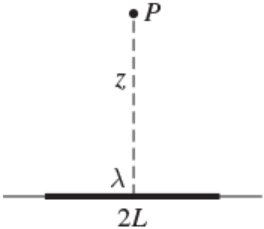
\includegraphics[width=2.08333in,height=\textheight]{Figures/L2_prob3.pdf}
\end{enumerate}

\textbf{Hint:} You may be tempted to use your result from Q5 of the
Lecture 1 problems, however it is easier to directly calulate the
potential here, by splitting up the line into infinitesimals segments
and summing over the potentials from all segments, working from the
formula for potential of a point charge.

\bookmarksetup{startatroot}

\chapter{Work and Energy in
Electrostatics}\label{work-and-energy-in-electrostatics}

\emph{Recommended reading}: Griffiths Section 2.4

\section{Work done to move a charge}\label{work-done-to-move-a-charge}

In general, the work done to move an electric charge is calculated in
the same way we calculate mechanical work when solving mechanics
problems, taking the form:

\$\$

W = \int \mathrm{\mathbf{F}} \cdot \mathrm{d} \mathrm{\mathbf{l}} 

\$\$

Let's say we have some configuration of source charges, and we want to
move a test charge past these charges, as represented in this diagram:

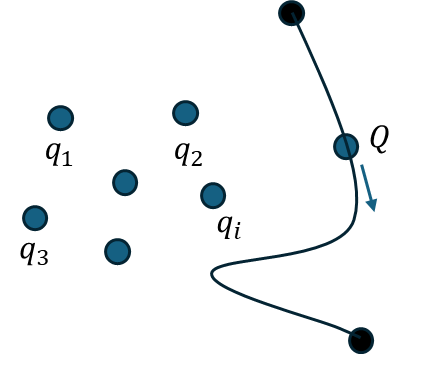
\includegraphics[width=3.125in,height=\textheight]{Figures/workdone_charge.png}

Let us work out how much work we need to do to move the charge along
this path. The work done to move a charge from point \textbf{a} to point
\textbf{b} is given by:

\$\$

W = \int\_\{\mathrm{\mathbf{b}}\}\^{}\{\mathrm{\mathbf{a}}\}
\mathrm{\mathbf{F}} \cdot \mathrm{d} \mathrm{\mathbf{l}} 

\$\$

Each of the charges is exerting a force
\(\mathrm{\mathbf{F}}= Q \mathrm{\mathbf{E}}\) on the test charge,
therefore the total work becomes:

\$\$

W = - Q \int\_\{\mathrm{\mathbf{b}}\}\^{}\{\mathrm{\mathbf{a}}\}
\mathrm{\mathbf{E}} \cdot \mathrm{d} \mathrm{\mathbf{l}} =
Q{[}V(\mathrm{\mathbf{b}}) - V(\mathrm{\mathbf{a}}){]}

\$\$

This equation re-states what we discussed in Lecture 2 - that the
potential difference between two points \(\mathrm{\mathbf{a}}\) and
\(\mathrm{\mathbf{b}}\) is the work done per unit charge to bring a
charge from point \(\mathrm{\mathbf{a}}\) to point
\(\mathrm{\mathbf{b}}\). If you want to bring a charge \(Q\) in from
very far away and place it at point \(\mathrm{\mathbf{r}}\), you the
work you have to do is

\[W = Q[V(\mathrm{\mathbf{r}}) - V(\infty)]\]

which, if you use a reference point at infinity, simply becomes

\[W = Q V(\mathrm{\mathbf{r}})\]

which should be a familiar expression from your previous studies.

\section{Energy of a point charge
distribution}\label{energy-of-a-point-charge-distribution}

If you want to assemble a group of point charges, the work required to
do so is given by

\begin{equation}\phantomsection\label{eq-workMulti}{ W = \frac{1}{2} \sum_{i=1}^n q_i V(\mathrm{\mathbf{r}}_i) }\end{equation}

Let's break this down. To calculate the work done to assemble a group of
point charges, we need to first realise the fact that the first charge
to join the group does not take any work, because there is no electric
field present for it to interact with. It is only when we try to
introduce further charges to configuration that work needs to be done.
We therefore choose one of our charges arbitrarily to be the first
charge. For every subsequent charge that is brought in, the work done to
bring it in is proportional to \(q_i V(\mathrm{\mathbf{r}}_i)\), where
\(q_i\) is the charge in question and \(V(\mathrm{\mathbf{r}}_i)\) is
the potential at position \(\mathrm{\mathbf{r}}_i\) (position of
\(q_i\)) due to all the other charges that are present. Summing over all
of these will result in the work needed to add every charge to the
distribution, and therefore gives the potential energy of the whole
charge configuration. Summing the potentials of each charge with respect
to the rest of the group of charges will lead to each pair of charges
being considered twice, which is not physical, therefore the factor of
\(\frac{1}{2}\) is introduced to remove this problem. For a full
derivation and explanation of Equation~\ref{eq-workMulti}, see Griffiths
Section 2.4.2.

\section{Energy of a continuous charge
distribution}\label{energy-of-a-continuous-charge-distribution}

Now consider the situation where we have a continuous charge
distribution instead of a collection of point charges. It is important
to note here that a charge distribution is never truly continuous -
charge always comes in the form of discrete point charges such as
electrons, protons etc - however if we have a very large amount of point
charges we can consider them to be a continuous distribution with some
associated charge density. For a volume charge density,
Equation~\ref{eq-workMulti} becomes

\begin{equation}\phantomsection\label{eq-cont1}{ W = \frac{1}{2}\int \rho V \mathrm{d} \tau}\end{equation}

where \(V\) denotes volume and \(\mathrm{d} \tau\) is the infinitesimal
volume element.

The same formulation works for a surface charge density\ldots{}

\[ W = \frac{1}{2}\int \sigma V \mathrm{d} a\]

\ldots{} and a line charge density

\[ W = \frac{1}{2}\int \lambda V \mathrm{d} l\]

as well.

The energy of a continuous charge distribution can also be expressed in
the following way:

\[ W = \frac{\epilon_0}{2} \left( int_{\mathcal{V}} E^2 \mathrm{d} \tau + \oint_{\mathcal{S}} V \mathrm{\mathbf{E}}\cdot \mathrm{d} \mathrm{\mathbf{a}}\].\{\#eq-cont2\}

We will not look at the derivation for this now, because it involves
concepts not yet encountered in this course. After Lecture 7, I would
recommend that you look at Section 2.4.3 of the Griffiths for the
derivation of \textbf{?@eq-cont2}.

If we integrate \textbf{?@eq-cont2} over all space, the surface integral
goes to zero and we end up with:

\[ W = \frac{\epilon_0}{2} \int_{\mathrm{all \; space}} E^2 \mathrm{d} \tau \].\{\#eq-cont3\}

\section{Work and the electric
dipole}\label{work-and-the-electric-dipole}

\subsection{Electric dipole field}\label{electric-dipole-field}

First of all, let's talk about what an electric dipole is. An electric
dipole is a combination of a positive and negative charge, equal in
magnitude, a small distance from each other. A visual representation of
the electric field of a dipole is shown below:

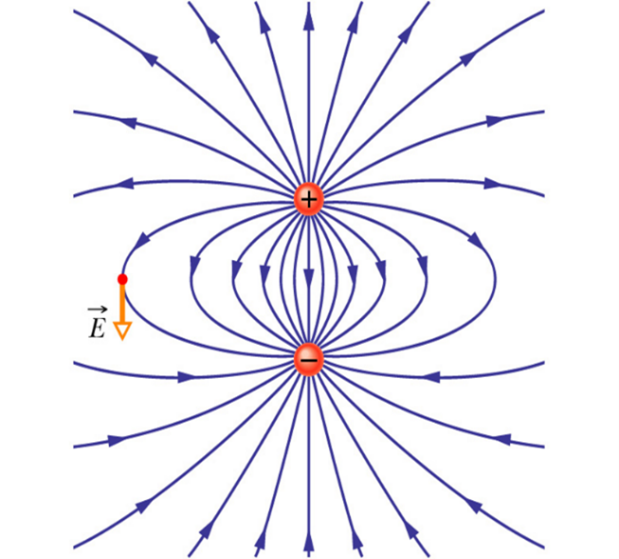
\includegraphics[width=3.125in,height=\textheight]{Figures/dipole_field.png}

The vector field for an electric dipole can be calculated by summing the
vector fields due to the two charges.

Let's consider the dipole in the diagram below. The dipole is oriented
along the \(y\)-axis, and we define an arbitrary point \(P\) on the
\(x\)-axis:

\begin{figure}[H]

{\centering 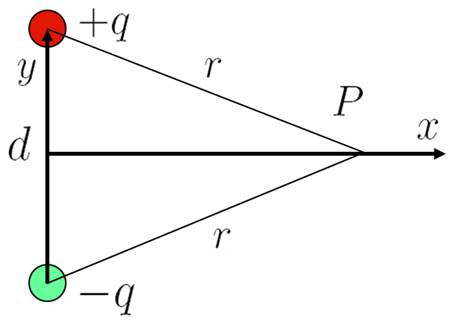
\includegraphics[width=3.125in,height=\textheight]{Figures/dipole_diagram.png}

}

\caption{A dipole represented in the \(x\)-\(y\) plane, where \(d\) is
the distance between the charges.}

\end{figure}%

For dipoles, we define a quantity known as the electric dipole moment,
given by \$\mathrm{\mathbf{p}} = q \mathrm{\mathbf{d}} \$. The electric
dipole moment is the product of the charge \(q\) (pay attention here!
This is the charge on
\bf{one of} the charges, not both added together) and $d$, which is the displacement vector pointing from the negative charge to the positive charge. Note that this is the opposite way to how electric fields are defined, which point from positive to negative charges.  

\begin{figure}[H]

{\centering 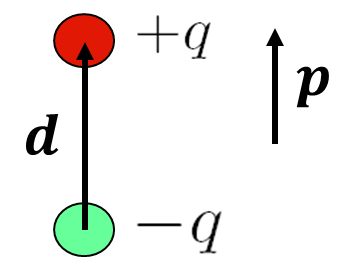
\includegraphics[width=3.125in,height=\textheight]{Figures/dipole_moment.png}

}

\caption{A diagram of an electric dipole, showing the vector quantities
\(\mathrm{\mathbf{d}}\) and \(\mathrm{\mathbf{p}}\), which are the
vector length of the dipole and the dipole moment, respectively.}

\end{figure}%

The field produced by the dipole at point \(P\) on the \(x\)-axis is
given by: \[
\mathrm{\mathbf{E}}= \frac{1}{4\pi \epsilon_0} \frac{qd}{ \left( x^2 \left( \frac{d}{2} \right)^2 \right)^{\frac{3}{2}} }
\]

Does this look familiar? If you attempted Q1 of the Problem Set for
Lecture 1, you have actually already calculated the electric field of an
electric dipole! The only difference is that in that question you
calculated the field at a point on the \(z\)-axis, but otherwise it
should be same mathematical expression. In that problem you were asked
to think about the dipole field in different ranges of values of \(z\).
If we look at the above expression, we can see that in the limit
\(x >> d\) (in other words, when we are at a distance \(x\) from the
dipole that is much larger than the size of the dipole \(d\)) the
electric field due to the dipole can be reduced to: \[
\mathrm{\mathbf{E}}= \frac{1}{4 \pi \epsilon_0} \frac{\mathrm{\mathbf{p}}}{x^3}
\]

So the field is very similar to that of a point charge, however it drops
off even faster with distance. If we look at the field lines of the
dipole, we can see how this happens - instead of spreading straight out
from the charges, the field lines bend towards the axis of the dipole,
therefore diverging faster than the point charge case.

\subsection{Energy of a dipole in an external electric
field}\label{energy-of-a-dipole-in-an-external-electric-field}

Now, back to the topic at hand: work and energy.

Consider a dipole that is placed within a uniform electric field. The
force on each charge has magnitude \(qE\), but since these forces are in
opposite directions there is no net force on the dipole. There is
however a torque about the centre of the dipole. See
\textbf{?@fig-dipoleExt} to get a feel for this.

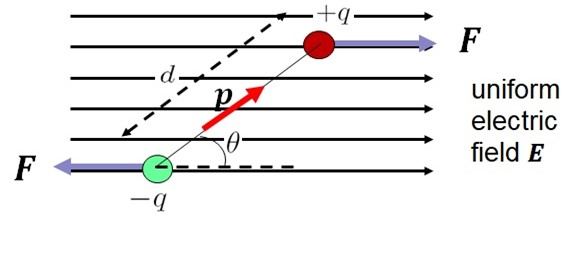
\includegraphics[width=4.16667in,height=\textheight]{Figures/dipole_extE.jpg}\{\#fig-dipoleExt\}

The torque about the centre of the dipole in \textbf{?@fig-dipoleExt} is

\[ \tau = 2 F \frac{d}{2} \sin\theta = qEd\sin\theta = p E \sin\theta \]

This can be expressed in vector form as
\[ \mathrm{\mathbf{\tau}} = \mathrm{\mathbf{p}}\times \mathrm{\mathbf{E}}\]

The torque will cause the dipole to rotate and align itself with the
electric field, as shown here:

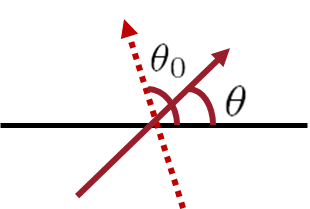
\includegraphics[width=3.125in,height=\textheight]{Figures/dipole_align.png}\{\#fig-dipoleAlign\}

If we think about it in terms of work - we Would have to do work on the
dipole to rotate it away from the position where it is aligned with the
electric field (which is when the positive charge is on the right). This
work is stored as potential energy. The dipole does work (in other words
it loses potential energy) rotating towards its aligned position.

The work done is the integral of the product of the torque and the angle
turned through:

\[
\begin{split} 
W & = \int_{\theta_0}^{\theta} \tau \mathrm{d} \theta \\
& = \int_{\theta_0}^{\theta} pE\sin\theta \mathrm{d} \theta \\
& = [-pE \cos \theta]_{\theta_0}^{\theta} 
\end{split}
\]

The change in potential energy is \(\Delta U = W\), hence:

\[ \Delta U = U(\theta_0) - U (\theta) = pE(\cos\theta_0 - \cos\theta) \]

The zero of potential energy \(U(\theta_0)\) can be chosen to be
anywhere, so we can choose it to correspond to \(\theta = 90^{\circ}\)
in which case \(U = -pE\cos\theta\).

Not surprisingly, the energy is at a minimum when the dipole is aligned
with the field, at which point the torque will be zero.

\section{Practice problems}\label{practice-problems-2}

\begin{enumerate}
\def\labelenumi{\arabic{enumi})}
\tightlist
\item
  As discussed in the lecture, consider a collection of 3 charges that
  form 3 sides of a square, as shown:
\end{enumerate}

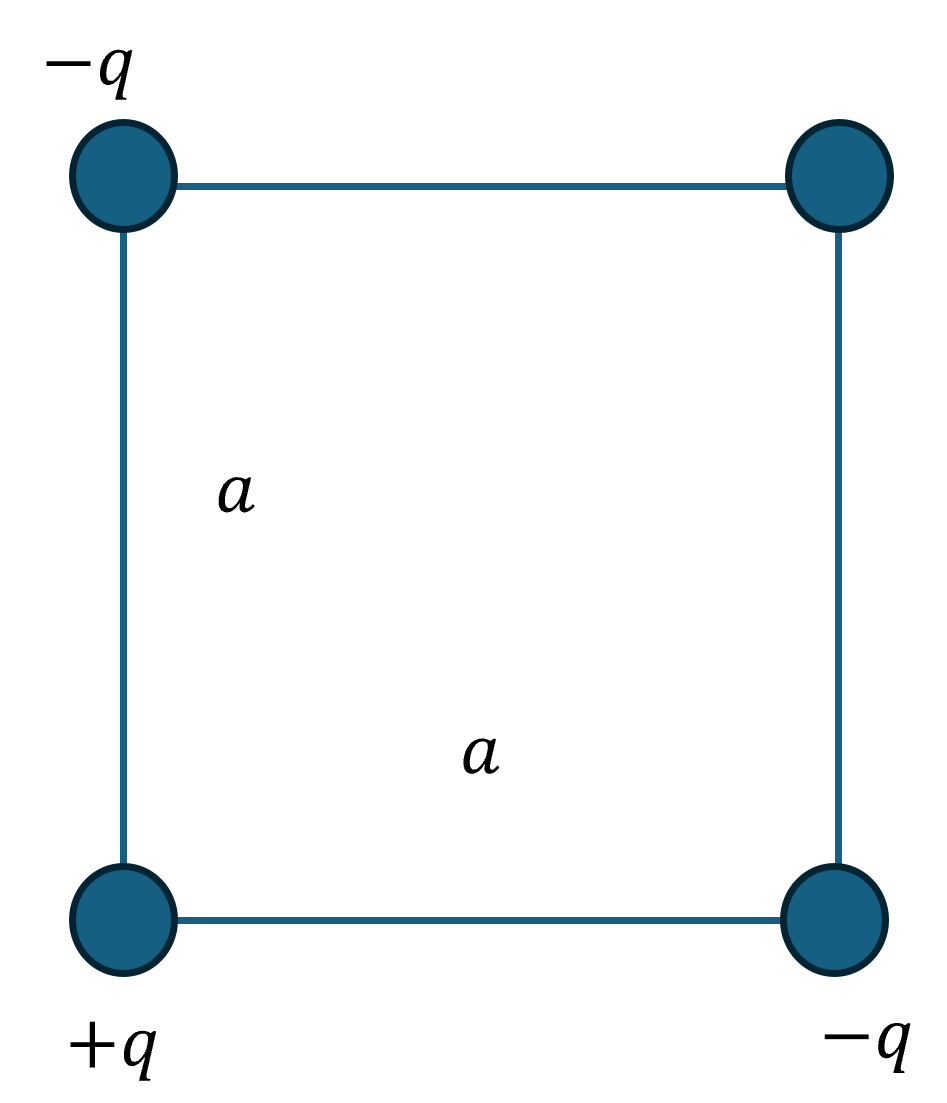
\includegraphics[width=2.08333in,height=\textheight]{Figures/L3_3charges.png}

In the lecture, we calculated the amount of work it takes to bring in a
4th charge \(+q\) from far away and place it in the 4th corner of the
square.

Calculate the total work it takes to assemble all 4 charges into the
square configuration.

\begin{enumerate}
\def\labelenumi{\arabic{enumi})}
\setcounter{enumi}{1}
\tightlist
\item
  (\emph{Griffiths Problem 2.35}) Find the energy stored in the
  uniformly charged solid sphere of radius \(R\) and charge \(q\). Do it
  3 different ways:
\end{enumerate}

\begin{enumerate}
\def\labelenumi{(\alph{enumi})}
\item
  Use the equation \$ W = \frac{1}{2} \int \rho V \mathrm{d} \tau \$.
  You found the potential in Q1 of the Lecture 1 Problem Set.
\item
  Use the equation \$ W = \frac{\epilon_0}{2}
  \int\_\{\mathrm{all space}\} E\^{}2 \mathrm{d} \tau \$. The electric
  field is given in Q1 of the Lecture 1 Problem Set.
\item
  Use the equation \$ W = \frac{\epilon_0}{2} \left(
  int\_\{\mathcal{V}\} E\^{}2 \mathrm{d} \tau + \oint\_\{\mathcal{S}\} V
  \mathrm{\mathbf{E}} \cdot \mathrm{d} \mathrm{\mathbf{a}} \$. Take a
  spherical volume of radius \(a\). What happens as
  \(a \rightarrow \infty\)?
\end{enumerate}

\bookmarksetup{startatroot}

\chapter{Magnetic Fields and the Lorentz Force
Law}\label{magnetic-fields-and-the-lorentz-force-law}

\emph{Recommended reading}: Griffiths Section 5.1

\section{Pre-lecture problem}\label{pre-lecture-problem-2}

(Griffiths, Problem 5.1)

This problem should help you revise some magnetism concepts from your
A-level course.

A particle of charge \(q\) enters a region of uniform magnetic field
\(\mathrm{\mathbf{B}}\) (pointing \emph{into} the page). The field
deflects the particle a distance \(d\) above the original line of
flight, as shown in the diagram below.

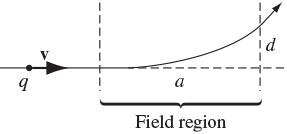
\includegraphics[width=2.08333in,height=\textheight]{Figures/L4_preprob.png}

\begin{enumerate}
\def\labelenumi{(\alph{enumi})}
\item
  Is the charge positive or negative?
\item
  In terms of \(a\), \(d\), \(B\), and \(q\), find the momentum of the
  particle.
\end{enumerate}

\section{Magnetic Fields}\label{magnetic-fields}

In electrostatics, we discussed electric charges as interacting via the
electric field. An electric field surrounds a charge, and when a second
charge is brought near to the first it interacts with the field,
experiencing a force. The electric field diverges from charges - all
charges are either a source or a sink for the electric field.

However, the magnetic field does not work in the same way. We cannot
think of ``magnetic charges'' interacting via the magnetic field,
because magnetic charges have not been found to exist - there is no
evidence for single North or South poles. Searches have been made for
magnetic monopoles, but without any success, although their existence
has not been entirely ruled out. (This is beyond our syllabus but if you
are interested you could try looking at
\href{https://royalsocietypublishing.org/doi/10.1098/rsta.2018.0328}{this
paper}.)

Magnetic fields, denoted by \(\mathrm{\mathbf{B}}\), are vector fields
that are produced by moving electric charges, for example electric
currents. The direction of the magnetic field at a given point in space
is the direction in which the north end of a compass needle would point
when placed at that point.

There are some important differences between the behaviour of charges in
electric and magnetic fields. In electric fields, the force on a charge
is parallel to the field lines -- a positive charge moves along the
field lines in the direction indicated. In magnetic fields, the force on
a moving charge is perpendicular to the field lines.

As with the electric field, the magnetic field can be represented using
field lines and the density of field lines represents the strength of
the field. The direction of the magnetic field at a given point in space
is defined as the direction in which a compass needle would point if
placed at this point. In other words, it is the direction in which the
North pole of a magnetic would move (i.e.~away from another North pole).
The direction of the magnetic field due to an electric current is given
by the right-hand rule. If you point the thumb of your right hand in the
direction of the current and then curl the fingers the field is in the
direction of the curl of your fingers.

In the same way as the electric field, the strength (or in other words,
the magnitude) of the magnetic field is usually indicated by the density
of the field lines. Magnetic field strength is measured in the SI unit
of Tesla (T) or in Gauss, where 1 Tesla = \(10^4\) Gauss.

\begin{figure}[H]

{\centering 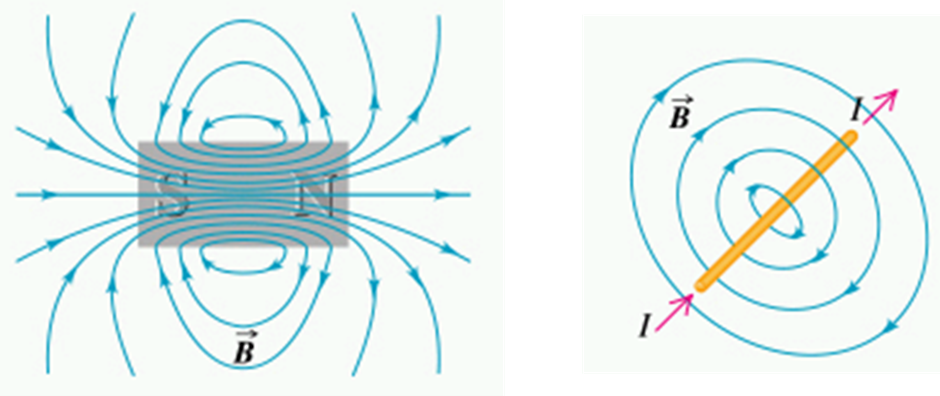
\includegraphics[width=5.20833in,height=\textheight]{Figures/MagFields.png}

}

\caption{\emph{Left:} The magnetic field produced by a bar magnet.
\emph{Right:} Section of a wire (yellow) carrying current \(I\) and the
magnetic field \(\mathrm{\mathbf{B}}\) that it produces.}

\end{figure}%

Magnetic field lines always form closed loops whereas electric field
lines begin and end on charges. As magnetic field lines are closed
loops, all field lines entering a closed surface must leave it as well -
therefore the net magnetic flux through any surface is zero.

\subsection{The Lorentz Force Law}\label{the-lorentz-force-law}

As we have seen in the previous lectures on electrostatics, electric
charges exert forces on one another as a result of the electric fields
that arise from them. In the same way, a magnetic field exerts a force
on a moving charge, because the moving charge produce its own magnetic
field and the two fields interact, producing a force.

The magnetic force on a moving charge is given by

\[
\mathrm{\mathbf{F}}_B = q(\mathrm{\mathbf{v}}\times \mathrm{\mathbf{B}}) {#eq-lorentz}
\]

The term \(\mathrm{\mathbf{v}}\times \mathrm{\mathbf{B}}\) represents
the cross product of the velocity and magnetic field vectors. As you
will know, the cross product of two vectors results in a vector that is
perpendicular to both. Therefore, the direction of
\(\mathrm{\mathbf{F}}\) is perpendicular to both \(\mathrm{\mathbf{v}}\)
and \(\mathrm{\mathbf{B}}\). You will also know that the cross product
of two vectors \(\mathrm{\mathbf{a}}\) and \(\mathrm{\mathbf{b}}\) is
equal to \(ab \sin\theta\). Hence, the magnitude of the magnetic force
is given by:

\[
F_B = qvB \sin\theta
\]

This is not the full picture, however. The \textbf{Lorentz Force Law}
describes the total force on a moving charge, including the effect of
both electric and magnetic fields. The force \(\mathrm{\mathbf{F}}\)
experienced by a charge \(q\) moving with a velocity
\(\mathrm{\mathbf{v}}\) in an electric field \(\mathrm{\mathbf{E}}\) and
a magnetic field \(\mathrm{\mathbf{B}}\) is given by:

\[
\mathrm{\mathbf{F}}= q(\mathrm{\mathbf{E}}+ \mathrm{\mathbf{v}}\times \mathrm{\mathbf{B}})
\]

The Lorentz force law is responsible for the circular motion of charged
particles in magnetic fields, as represented in the figure below:

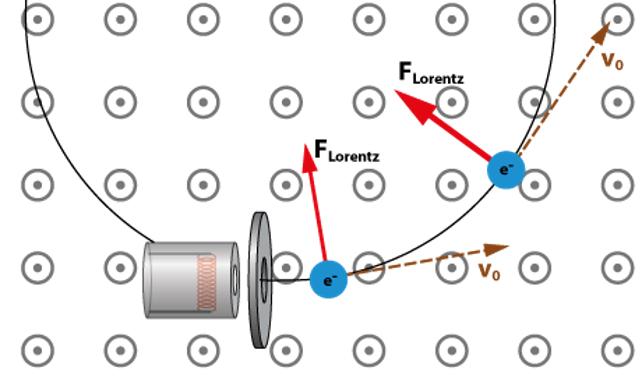
\includegraphics[width=5.20833in,height=\textheight]{Figures/lorentz_motion.png}

The centripetal force required for circular motion is supplied by the
magnetic force. This principle is used in cyclotrons and other particle
accelerators.

The Lorentz force law also leads to the Hall effect, which is the
development of a transverse electric field in a solid material when it
carries an electric current and is placed in a magnetic field that is
perpendicular to the current.

\section{Magnetic field of currents}\label{magnetic-field-of-currents}

As we mentioned earlier, currents are moving charges and therefore they
also experience a force in the prescence of a magnetic field. We can use
the Lorentz force law to work out what this force will be. Here we
consider a current as a moving line charge with velocity
\(\mathrm{\mathbf{v}}\) and linear charge density \(\lambda\). The
current in the wire is given by \(I = \lambda \mathrm{\mathbf{v}}\) -
you should be able to see upon inspection that this makes sense
dimensionally, but check out Griffiths 5.1.3 for a more detailed
derivation. If we think of the current as being made up of infinitesimal
charges \(\mathrm{d} q\), integrating to sum all of these across the
length of the wire would give the total charge in the wire. Hence, by
analogy to \textbf{?@eq-lorentz}, the force on the wire would be

\begin{equation}\phantomsection\label{eq-currentforce}{ \mathrm{\mathbf{F}}_{mag} = \int (\mathrm{\mathbf{v}}\times \mathrm{\mathbf{B}}) \mathrm{d} q }\end{equation}

We can express \(\mathrm{d}q\) as \(\lambda \mathrm{d} l\), hence the
magnetic force becomes

\begin{equation}\phantomsection\label{eq-currentforce2}{ \ begin{split} 
\mathrm{\mathbf{F}}_{mag} &= \int (\mathrm{\mathbf{v}}\times \mathrm{\mathbf{B}}) \lambda \mathrm{d} l \\
&= \int (\mathrm{\mathbf{I}}\times \mathrm{\mathbf{B}}) \mathrm{d} l 
\end{split}
}\end{equation}

\(\mathrm{\mathbf{I}}\) and \(\mathrm{d} \mathrm{\mathbf{l}}\) point in
the same direction, therefore it is valid to express
Equation~\ref{eq-currentforce2} as

\begin{equation}\phantomsection\label{eq-currentforce3}{ \mathrm{\mathbf{F}}_{mag} &= \int I (\mathrm{d} \mathrm{\mathbf{l}}\times \mathrm{\mathbf{B}}) }\end{equation}

Equation~\ref{eq-currentforce3} is the generally accepted way to express
the magnetic force on a segment of current-carrying wire, and will be
used in this form in this course. However,
Equation~\ref{eq-currentforce3} models a current-carrying wire as a
1-dimensional line charge, which of course in reality it is not. If we
want to be more realistic and calculate the magnetic force on a volume
current (so, considering the current in a 3-dimensional wire) the
magnetic force is

\begin{equation}\phantomsection\label{eq-currentforceVol}{ \mathrm{\mathbf{F}}_{mag} &= \int (\mathrm{\mathbf{v}}\times \mathrm{\mathbf{B}}) \rho \mathrm{d}\tau = \int (\J \times \mathrm{\mathbf{B}}) \mathrm{d}\tau }\end{equation}

where \(\mathrm{d}\tau\) is the volume element, \(\rho\) is the volume
charge density and \(\J = \rho \mathrm{\mathbf{v}}\) is the volume
current density. The volume current density is defined as the current
per unit area for the area perpendicular to the current flow
(essentially the cross-sectional area of the wire). Once again,
Griffiths 5.1.3 is worth reading if you want a more detailed derivation.

\section{Work done by magnetic
fields?}\label{work-done-by-magnetic-fields}

\section{Practice problems}\label{practice-problems-3}

\begin{enumerate}
\def\labelenumi{\arabic{enumi})}
\tightlist
\item
  In the lecture we sketched and calculated the trajectory of the
  particle in Griffiths Example 5.2, in the case where the particle was
  released from the origin at zero velocity (see the lecture slides on
  Blackboard if you were not in attendance).
\end{enumerate}

Find and sketch the trajectory of the particle in Example 5.2, if it
starts at the origin with velocity: (a)
\((E/B) \hat{\mathrm{\mathbf{y}}}\) (b)
\((E/2B) \hat{\mathrm{\mathbf{y}}}\) (c)
\((E/B) (\hat{\mathrm{\mathbf{y}}} + \hat{\mathrm{\mathbf{z}}}\))

\begin{enumerate}
\def\labelenumi{\arabic{enumi})}
\setcounter{enumi}{1}
\tightlist
\item
  (\emph{Griffiths Problem 5.3})
\end{enumerate}

In 1897, J. J. Thomson ``discovered'' the electron by measuring the
charge-to-mass ratio of ``cathode rays'' (actually, streams of
electrons, with charge \(q\) and mass \(m\)) as follows:

\begin{enumerate}
\def\labelenumi{(\alph{enumi})}
\item
  First he passed the beam through uniform crossed electric and magnetic
  fields \(\mathrm{\mathbf{E}}\) and \(\mathrm{\mathbf{B}}\) (mutually
  perpendicular, and both of them perpendicular to the beam), and
  adjusted the electric field until he got zero deflection. What was the
  speed of the particles in terms of \(E\) and \(B\) when he reached
  zero deflection?
\item
  Then he turned off the electric field, and measured the radius of
  curvature, \(R\), of the beam, as deflected by the magnetic field
  alone. In terms of \(E\), \(B\), and \(R\), what is the charge-to-mass
  ratio (\(q/m\)) of the particles?
\end{enumerate}

\bookmarksetup{startatroot}

\chapter{The Biot-Savart Law}\label{the-biot-savart-law}

\emph{Recommended reading}: Griffiths Section 5.2

\section{Pre-lecture problem}\label{pre-lecture-problem-3}

Find the magnitude of the attractive force between two long, parallel
wires which are a distance \(d\) apart, carrying currents \(I_1\) and
\(I_2\).

We saw in the last lecture that a current-carrying wire experiences a
magnetic force when in the prescence of an applied magnetic field, and
we found an expression for the magnetic force on a segment of
current-carrying wire. Ultimately, current-carrying wires experience
this force because they produce their own magnetic field which interacts
with the applied magnetic field. The Biot-Savart Law is a formula for
the magnetic field of a steady line current. Note that we are once again
thinking about \emph{line} currents, so we are modelling our currents as
1-dimensional.

\textbf{An aside on steady currents:} The Biot-Savart Law only applies
to so-called ``steady currents''. A steady current is defined as a
continuous flow of charge that goes on forever, without changing and
without charge piling up anywhere. In reality, there is no such current,
but for the purposes of this course we can model current-carrying wires
as carrying steady currents. If the current wasn't a steady current, the
magnetic field produced by the current would be varying as a function of
time, and we would no longer be in the realm of magnetostatics, which
deals in static (non-time varying) magnetic fields.

The Biot-Savart Law takes the following form:

\[\mathrm{\mathbf{B}}(\mathrm{\mathbf{r}}) = \frac{\mu_0}{4\pi} \int \frac{\mathrm{\mathbf{I}}\times \hat{\mathrm{\mathbf{r}}_s} }{\mathrm{\mathbf{r}}_s^2} \mathrm{d}l' =  \frac{\mu_0}{4\pi} \int I \frac{\mathrm{d} \mathrm{\mathbf{l}}' \times \hat{\mathrm{\mathbf{r}}_s} }{\mathrm{\mathbf{r}}_s^2} \]

In your previous studies you may have come across the formula for the
magnetic field at a distance from a current-carrying wire. Have you ever
wondered where this equation came from? Turns out it is derived using
the Biot-Savart Law - I'm going to guide you the derivation here, to
demonstrate how we use the Biot-Savart Law.

\section{Magnetic Field of a Current-Carrying
Wire}\label{magnetic-field-of-a-current-carrying-wire}

Our task here is to find the magnetic field at a distance \(s\) from a
long, straight wire carrying a steady current \(I\).

\textbf{Important:} When we talk about a ``long'' wire, we are talking
about a wire that is so long that it can be considered infinitely long -
so that we can assume it carries a steady current (see ``aside on steady
currents'' above). In real life, wires that carry currrent are usually
part of a closed circuit, so we can consider most current-carrying wires
to be carrying steady currents, as the current in closed circuit will go
on forever (until a switch is opened, a battery dies, a component
breaks, and so on\ldots).

Let us first visualise the problem with a diagram:
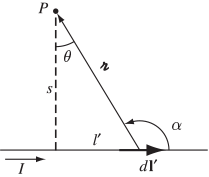
\includegraphics[width=2.08333in,height=\textheight]{Figures/BS-example-1.png}\{\#BS-ex1\}

This figure is taken from the Griffiths, therefore the curly ``r''
pointing from \(\mathrm{d} \mathrm{\mathbf{l}}'\) to \(P\) should be
interpreted as \(\mathrm{\mathbf{r}}_s\) in our notation. As a reminder,
the Biot-Savart Law is given by

\[\mathrm{\mathbf{B}}(\mathrm{\mathbf{r}}) =  \frac{\mu_0}{4\pi} \int I \frac{\mathrm{d} \mathrm{\mathbf{l}}' \times \hat{\mathrm{\mathbf{r}}_s} }{\mathrm{\mathbf{r}}_s^2} \]

In (\textbf{BS-ex1?}),
\(\mathrm{d} \mathrm{\mathbf{l}}' \times \hat{\mathrm{\mathbf{r}}_s}\)
points out of the page (because it must be perpendicular to both
vectors) and has magnitude \(\mathrm{d} l' \sin\alpha\). However, it is
more convenient in this problem for us to to work with the angle
\(\theta\), because we can use trigonometric identities to relate
\(\theta\) more easily to the other variables in our problem. Therefore
we can use the angle addition formula
\(\sin(A + B) = \sin A \cos B + \cos A \sin B\), to find
\[ \sin\alpha = \sin(90 + \theta) = \sin(90)\cos\theta + \cos(90)\sin\theta = \cos\theta \]

Hence, the magnitude of
\(\mathrm{d} \mathrm{\mathbf{l}}' \times \hat{\mathrm{\mathbf{r}}_s}\)
is

\[ \mathrm{d} l' \cos\theta \]

We can also say that \(l' = s \tan\theta\), therefore

\[ \begin{split} 
\frac{\mathrm{d} l'}{\mathrm{d} \theta} &=  \frac{\mathrm{d} }{\mathrm{d} \theta} s \tan\theta \\
\mathrm{d}l' &=  \frac{s}{ \cos^2 \theta} \mathrm{d}\theta
\end{split}
\]

Finally, we can see that \(s = r_s \cos \theta\), so we can state

\[ \frac{1}{\mathrm{\mathbf{r}}_s^2} = \frac{\cos^2 \theta}{s^2} \]

We now have everything we need to compute the integral in the
Biot-Savart Law. We can integrate with respect to \(\theta\), and find
the integral between two angles \(\theta_1\) and \(\theta_2\), as
represented in this figure:

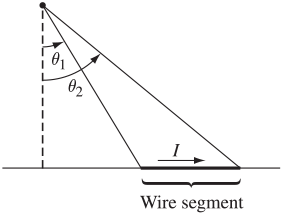
\includegraphics[width=2.08333in,height=\textheight]{Figures/BS-example-2.png}

Therefore

\[ \begin{split} 
B &= \frac{\mu_0 I}{4 \pi} \int_{\theta_1}^{\theta_2} \left( frac{\cos^2 \theta }{s^2} \right) \left( \frac{s}{\cos^\theta} \right) \cos\theta \mathrm{d}\theta   \\
 &= \frac{\mu_0 I}{4 \pi s} \int_{\theta_1}^{\theta_2}  \cos\theta \mathrm{d}\theta \\
 &= \frac{\mu_0 I}{4 \pi s} (\sin\theta_2 - \sin \theta_1) 
\end{split}
\]

The above equations represents the \(B\)-field at a distance \(s\) from
a short section of wire between two arbitrary anglular positions
\(\theta_1\) and \(\theta_2\). This is not physical however, because a
short section of wire cannot carry a steady current. Therefore let's
think about what happens when we extend the length of the wire to
infinity. For an infinitely long wire, \(\theta_1 = -\pi/2\) and
\(\theta_2 = \pi/2\). Hence, the magnitude of the \(B\)-field at a
distance \(s\) from a long current-carrying wire is

\[ B = \frac{\mu_0 I}{2\pi s}. \]\#eq-Bwire

If you didn't manage the pre-lecture problem, try it again now using
what you have learned in this lecture.

\section{Practice problems}\label{practice-problems-4}

\begin{enumerate}
\def\labelenumi{\arabic{enumi})}
\tightlist
\item
\item
\item
\end{enumerate}

\bookmarksetup{startatroot}

\chapter{Magnetic Vector Potential}\label{magnetic-vector-potential}

\emph{Recommended reading}: Griffiths Section 5.4

\emph{A problem to try before attending the lecture}: Griffiths Problem
1.18

\section{Practice problems}\label{practice-problems-5}

\bookmarksetup{startatroot}

\chapter{Gauss's Law}\label{gausss-law}

\emph{Recommended reading}: Griffiths Section 2.2

\#\#Pre-lecture problem

\section{Introduction}\label{introduction}

Gauss's Law is the first of Maxwell's equations and forms part of the
basis of classical electromagnetism. It concerns the relationship
between electric flux through a closed surface and the electric charge
enclosed within that surface. Crucially, it allows us a much simpler
method by which to calculate the electric field compared to

\section{Electric flux}\label{electric-flux}

In order to discuss Gauss's Law, we will now revisit the topic of
electrostatics, in particular electric fields. Consider again the
electric field of a point charge \(q\) at the origin. Imagine we
surround the charge by a spherical surface, centred on the origin with
radius \(R\). The area of the surface is \(A = 4\pi R^2\) , and the
magnitude of electric field a distance \(R\) from the charge is

\[ E(R) = \frac{q}{4\pi \epsilon_0 R^2} \],

with its direction perpendicular to the surface of the sphere.

We now introduce a new concept, known as the electric flux, which is the
flux of the electric field through a surface. It counts how many field
lines pierce the surface. In the case of the point charge, the flux
\(\Phi_E\) is given by the magnitude of the electric field multiplied by
the area of the surface, hence \(\Phi_E = EA\). In the case where we
have a point charge enclosed within the surface:

\[ \Phi_E = EA = \frac{q}{4\pi\epsilon_0 R^2} 4\pi R^2 = \frac{q}{\epsilon_0} \]

Notice how \(EA\) does not depend on the radius \(R\)! To understand
this, first let's generalise this concept beyond a spherical surface.
Let's say we deform the spherical surface into any other closed surface
(i.e., not tearing holes in it). Once a field line goes through the
surface, it counts towards the flux. No matter how big or small we make
the surface, and no matter its shape, the number of field lines coming
out of the surface will be the same provided that amount of charge
inside stays the same. If we add more charge inside, there will be a
higher density of field lines, hence more field lines will pierce the
surface. This means that the electric flux through a surface is a
measure of the amount of charge inside that surface, hence
\(\Phi_E = \frac{q}{\epsilon_0}\). As we can see, it is actually
\emph{proportional} to the amount of charge, modified by a constant
factor of \(\frac{1}{\epsilon_0}\). We can make sense of this
conceptually by reminding ourselves that \(\epsilon_0\) defines the
capacity of free space to hold electric fields, so it is sensible that
it should have a bearing on electric flux.

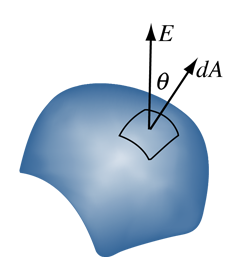
\includegraphics[width=3.125in,height=\textheight]{Figures/Gauss-surface-vector.png}\{\#surface-vector\}

In the case of a point charge and a spherical surface, the electric
field lines are always perpendicular to the surface. What happens when
the electric field is not perpendicular to the surface? Then we can
consider the projection of the surface perpendicular to \(E\). If the
angle between the field direction and the normal to the surface is θ, as
represented in (\textbf{surface-vector?}), then the flux of a constant
electric field of magnitude (i.e., field line density) \(E\) is
\(\Phi_E = EA \cos\theta\). If we have a volume V enclosed by a surface
S, we can ``tile'' S with infinitesimal tiles dA, where the area is
infinitesimally small, and the direction is out of the volume. The total
flux is then the sum over all the infinitesimal fluxes through dA. This
is a surface integral, written by ΦE = I S E · dA , (23) where the
symbol H S denotes integration over the entire surface S. Since field
lines cannot cross each other, if we have a bunch of charges inside the
volume V, the flux of the charges adds up. Positive charges create field
lines going out of the volume, and negative charges create field lines
going into the volume. Moreover, every field line sprouting at a
positive charge which does not exit V must terminate on a negative
charge inside V, cancelling that part of the flux for both charges.
Then, from Equation (20), we find that the flux through S is equal to
the total charge Qinside inside S, divided by 0: I S E · dA = Qinside 0
. (24) This is called Gauss' law. In the next lecture we will see how
this law can be used to calculate the electric field for some
interesting charge distributions.

Gauss' law in mathematical form looks pretty terrifying: I S E · dA =
Qinside 0 . (25) The power of this expression lies in the fact that it
is universally valid. So we would like to take this law as our starting
point in solving electrostatic problems. The way we use this equation is
by carefully unpacking the dot product in the integral, and choosing a
surface that we can easily integrate over, preferably without actually
having to solve the integral. First, let's see how we can calculate the
electric field of a point charge by starting from Gauss' law, just to
illustrate its use. We have the dot product E · dA, which we may get rid
Electricity 9 of by choosing a surface2 that either turns it into E · dA
= EdA or E · dA = 0. So we want to find a surface S that is either
parallel or perpendicular to the field, such that cos θ = 1 or cos θ =
0. The surface S may have different facets that are parallel and
perpendicular to the field. Next, we should consider the symmetry of the
problem. The point charge has spherical symmetry around the charge, so
the electric field must point radially outwards (or inwards). We're not
using knowledge of Equation (6) here, we deduce that any other direction
of the electric field would violate the symmetry of the problem. Knowing
the direction of the field allows us to choose S parallel to this, and
that determines the spherical surface of radius r. Any r will do. The
second observation from symmetry is that the magnitude of E must be
constant on S. Therefore, we find that for the integral we have I S E ·
dA = I S E dA = E I S dA , (26) where we pulled E out of the integral,
since it is constant over the entire surface S. Now we are left with
only the surface integral H S dA. But this is simply the surface area of
a sphere of radius r. Gauss' law then becomes I S E · dA = 4πr2E = q 0 .
(27) Rearranging gives the magnitude: E = q 4πr2 0 , (28) and including
the field direction we find the required Equation (6). In summary,
solving Gauss' law to find the electric field for a charge distribution
relies on symmetry arguments to find the direction of the field, which
in turn leads to the most convenient Gaussian surface S. Then you
evaluate the dot product E · dA, and solve the integral. Gauss' law is
one of the four Maxwell equations (in integral form) that completely
describes how electric and magnetic fields behave, even in situations
where there are no symmetries and the integral is really hard to
evaluate.

\section{Practice problems}\label{practice-problems-6}

\bookmarksetup{startatroot}

\chapter{Ampere's Law and Solenoids}\label{amperes-law-and-solenoids}

\newcommand{\l}{\mathrm{\mathbf{l}}}
\newcommand{\E}{\mathrm{\mathbf{E}}}
\newcommand{\F}{\mathrm{\mathbf{F}}}
\newcommand{\r}{\mathrm{\mathbf{r}}}

\newcommand{\x}{\mathrm{\mathbf{x}}}
\newcommand{\y}{\mathrm{\mathbf{y}}}
\newcommand{\z}{\mathrm{\mathbf{z}}}

\emph{Recommended reading}: Griffiths Section 5.3

\emph{A problem to try before attending the lecture}: Griffiths
{[}insert problem no.{]}

\bookmarksetup{startatroot}

\chapter{Faraday's Law and Lenz's Law}\label{faradays-law-and-lenzs-law}

\newcommand{\l}{\mathrm{\mathbf{l}}}
\newcommand{\E}{\mathrm{\mathbf{E}}}
\newcommand{\F}{\mathrm{\mathbf{F}}}
\newcommand{\r}{\mathrm{\mathbf{r}}}

\newcommand{\x}{\mathrm{\mathbf{x}}}
\newcommand{\y}{\mathrm{\mathbf{y}}}
\newcommand{\z}{\mathrm{\mathbf{z}}}

\emph{Recommended reading}: Griffiths Section 7.2.1 \& 7.2.2 (for some
bonus reading - check out 7.13)

\emph{A problem to try before attending the lecture}: Griffiths
{[}insert problem no.{]}

\bookmarksetup{startatroot}

\chapter{Maxwell's Equations in Free
Space}\label{maxwells-equations-in-free-space}

\newcommand{\l}{\mathrm{\mathbf{l}}}
\newcommand{\E}{\mathrm{\mathbf{E}}}
\newcommand{\F}{\mathrm{\mathbf{F}}}
\newcommand{\r}{\mathrm{\mathbf{r}}}

\newcommand{\x}{\mathrm{\mathbf{x}}}
\newcommand{\y}{\mathrm{\mathbf{y}}}
\newcommand{\z}{\mathrm{\mathbf{z}}}

\emph{Recommended reading}: Griffiths Section 7.3.1 - 7.3.4

\bookmarksetup{startatroot}

\chapter{Magnetisation and
Polarisation}\label{magnetisation-and-polarisation}

\newcommand{\l}{\mathrm{\mathbf{l}}}
\newcommand{\E}{\mathrm{\mathbf{E}}}
\newcommand{\F}{\mathrm{\mathbf{F}}}
\newcommand{\r}{\mathrm{\mathbf{r}}}

\newcommand{\x}{\mathrm{\mathbf{x}}}
\newcommand{\y}{\mathrm{\mathbf{y}}}
\newcommand{\z}{\mathrm{\mathbf{z}}}

\section{Polarisation}\label{polarisation}

\emph{Recommended reading}: Griffiths Section 4.1 - 4.3

\section{Magnetisation}\label{magnetisation}

\emph{Recommended reading}: Griffiths Section 6.1 - 6.3 (for some bonus
reading - check out 6.4)

\bookmarksetup{startatroot}

\chapter{Maxwell's Equations in
Matter}\label{maxwells-equations-in-matter}

\newcommand{\l}{\mathrm{\mathbf{l}}}
\newcommand{\E}{\mathrm{\mathbf{E}}}
\newcommand{\F}{\mathrm{\mathbf{F}}}
\newcommand{\r}{\mathrm{\mathbf{r}}}

\newcommand{\x}{\mathrm{\mathbf{x}}}
\newcommand{\y}{\mathrm{\mathbf{y}}}
\newcommand{\z}{\mathrm{\mathbf{z}}}

\emph{Recommended reading}: Griffiths Section 7.3.5 - 7.3.6 (for some
bonus reading, check out 7.4)

\bookmarksetup{startatroot}

\chapter{Capacitors and Inductors}\label{capacitors-and-inductors}

\newcommand{\l}{\mathrm{\mathbf{l}}}
\newcommand{\E}{\mathrm{\mathbf{E}}}
\newcommand{\F}{\mathrm{\mathbf{F}}}
\newcommand{\r}{\mathrm{\mathbf{r}}}

\newcommand{\x}{\mathrm{\mathbf{x}}}
\newcommand{\y}{\mathrm{\mathbf{y}}}
\newcommand{\z}{\mathrm{\mathbf{z}}}

\section{Capacitors}\label{capacitors}

\emph{Recommended reading}: Griffiths Section 4.4; Tipler \&
Mosca\ldots{}

\section{Inductors}\label{inductors}

\emph{Recommended reading}: Griffiths Section 7.2.3 \& 7.2.4; Tipler \&
Mosca\ldots{}

\bookmarksetup{startatroot}

\chapter{Circuits}\label{circuits}

\newcommand{\l}{\mathrm{\mathbf{l}}}
\newcommand{\E}{\mathrm{\mathbf{E}}}
\newcommand{\F}{\mathrm{\mathbf{F}}}
\newcommand{\r}{\mathrm{\mathbf{r}}}

\newcommand{\x}{\mathrm{\mathbf{x}}}
\newcommand{\y}{\mathrm{\mathbf{y}}}
\newcommand{\z}{\mathrm{\mathbf{z}}}

\emph{Recommended reading}: Griffiths Section 7.1.1 \& 7.1.2; Tipler \&
Mosca\ldots{}

\bookmarksetup{startatroot}

\chapter{}\label{section}

\newcommand{\l}{\mathrm{\mathbf{l}}}
\newcommand{\E}{\mathrm{\mathbf{E}}}
\newcommand{\F}{\mathrm{\mathbf{F}}}
\newcommand{\r}{\mathrm{\mathbf{r}}}

\newcommand{\x}{\mathrm{\mathbf{x}}}
\newcommand{\y}{\mathrm{\mathbf{y}}}
\newcommand{\z}{\mathrm{\mathbf{z}}}

Impedance

\emph{Recommended reading}: Tipler \& Mosca\ldots{}

\bookmarksetup{startatroot}

\chapter{Summary}\label{summary-2}

In summary, this book has no content whatsoever.

\bookmarksetup{startatroot}

\chapter*{References}\label{references}
\addcontentsline{toc}{chapter}{References}

\markboth{References}{References}

\phantomsection\label{refs}
\begin{CSLReferences}{0}{1}
\end{CSLReferences}



\end{document}
